\subsection{Presentation}
AutoML is a tool for choosing the best model (or ensemble) for fitting and predicting a dataset.\\
If using scikit-learn, the proper toolkit is defined as \href{https://automl.github.io/auto-sklearn/}{auto-sklearn}.

\subsection{Obtaining the Model}
Simply fitting the training data to the AutoSklearnClassifier gives us an "optimal" model.\\
In this case (shown by \emph{running model.show\_models}()), the result is an ensemble of several ensembles, involving SVMs, Random Forests, etc.

\subsection{AutoML vs Voting Classifier}
We achieved highest accuracy with the Voting Classifier, below is the ROC plot of the Voting classifer vs AutoML

\begin{center}
    \captionsetup{type=figure}
    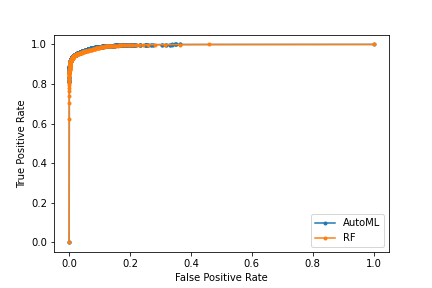
\includegraphics[width=250px]{AUC_automl.png}
    \captionof{figure}{RF vs AutoML}
\end{center}